\section{Consuntivi}
In questa sezione viene riportato il prospetto economico di ogni macro-fase conclusa, che evidenzia la differenza tra le spese previste e quelle effettivamente sostenute.

\subsection{Progettazione Architetturale}
Nella stesura iniziale del piano è stato largamente sottovalutato il tempo necessario per acquisire le conoscenze atte a chiarire come saranno strutturati i componenti e le classi del prodotto. Questo ha portato a non rispettare le date di consegna per la prima Revisione di Progettazione, e a spostare tutte le successive consegne alla prossima data disponibile. \\
Si è cercato nel migliore dei modi di chiarire quale parte di questo studio fosse rivolta all'apprendimento delle tecnologie adottate, e quindi a carico del gruppo, e quale invece riguardasse la creazione di una visione di insieme dei componenti di Premi, parte cruciale nella stesura della Specifica Tecnica: ne è risultata una diminuzione delle ore di lavoro dei progettisti, che si sono potuti dedicare alla stesura di altre parti del documento. \\
L'esito della Revisione dei Requisiti ha portato ad uno studio non previsto di nuove funzionalità, con un inevitabile aumento delle ore di lavoro dedicate alla correzione dell'Analisi dei Requisiti. \\
Le rimanenti attività si sono susseguite rispettando i tempi prestabiliti; la tabella sottostante mostra in verde le ore risparmiate e in rosso quelle non previste. \\

\begin{figure}[h]
\begin{center}
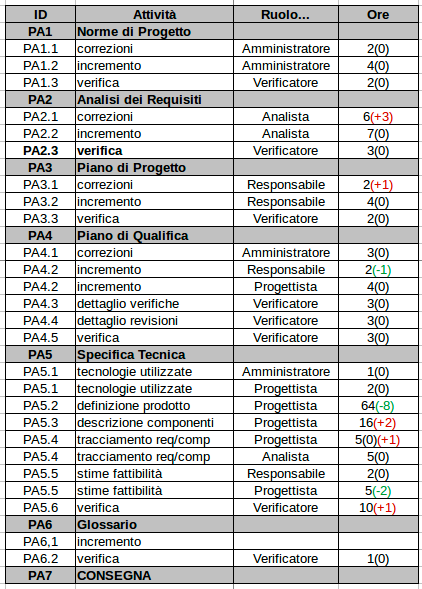
\includegraphics[scale=0.45]{img/consuntivo-progarc.png}
\caption{Tabella delle ore previste e sostenute nella Progettazione Architetturale.}
\end{center}
\end{figure}
\clearpage

\subsubsection{Conclusioni}
Dalla tabella precedente risulta una differenza di soli \textbf{2€} in questa macro-fase rispetto a quanto preventivato. \\ Lo studio delle tecnologie effettuato da tutti i membri del gruppo dovrebbe portare ad un risparmio di tempo nella prossima macro-fase, ma rimangono ancora da effettuare ulteriori approfondimenti sull'utilizzo di alcune librerie esterne. Pertanto non verranno per ora effettuati cambiamenti al prezzo concordato in precedenza.

\begin{figure}[h]
\begin{center}
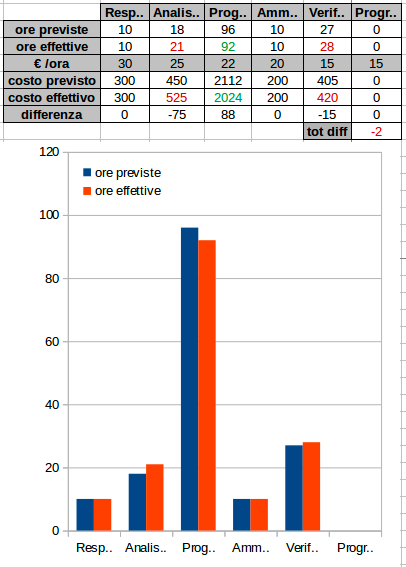
\includegraphics[scale=0.70]{img/consuntivo-progarc-tot.png}
\caption{Tabella dei costi totali previsti e sostenuti nella Progettazione Architetturale.}
\end{center}
\end{figure}
\clearpage




